\section{TCP sockets}\label{sec:tcp}

Without much surprise, all our Android applications use TCP.
\texttt{SOCK\_STREAM} sockets account for 73\% of all opened
sockets. 63\% of these TCP sockets \texttt{connect()} to a remote
address while 37\% do not call \texttt{connect()} or \texttt{connect()}
to a loopback address. We first briefly analyze these later sockets
that interact with local daemons or applications. We then
analyze in more details the sockets that connect to distant servers.

\subsection{Local sockets}

We observe that a staggering 73\% of the local sockets only call
\texttt{setsockopt(SO\_RCVTIMEO)} once or several times after the initial
\texttt{socket()} call. Since \texttt{SO\_RCVTIMEO} only modifies the receiving timeout of the target socket,
these operations seem wasteful but we could not find a valid explanation for
this behavior. Another 16\% of the local sockets only call \texttt{close()}
after \texttt{socket()} and 3\% call \texttt{ioctl(SIOCGIWNAME)} to determine
if the current interface is wireless before closing the socket.
Table~\ref{tab:tcp_sockets_usage} summarizes these findings. While 85\% of the
UDP sockets use \texttt{ioctl()} to retrieve information about the network, we
rarely observe \texttt{ioctl()} on TCP sockets. This supports our
observation that applications prefer to perform \texttt{ioctl()} requests
on UDP sockets because they are less costly.

\begin{table}[]
\centering
\begin{tabular}{ll}
\hline
\textbf{37\%} & \textbf{Local sockets}  \\ \hline
27\%                                & \texttt{setsockopt(SO\_RCVTIMEO)}          \\
6\%                                 & Immediate \texttt{close()}                 \\
3\%                                 & Determine if interface is wireless         \\
1\%                                 & Other usages                               \\ \hline
\textbf{63\%} & \textbf{Remote sockets} \\ \hline
59\%                                & Exchange data after \texttt{connect()}     \\
4\%                                 & Do not send/recv data from network
\end{tabular}
\caption{TCP sockets usage. \textmd{37\% do not connect()
or connect() to a loopback address while 63\% connect() to a remote address.
Most local sockets only call setsockopt(SO\_RCVTIMEO).}}
\label{tab:tcp_sockets_usage}
\end{table}

\subsection{Remotely connected sockets}

We now restrict our analysis to the 7505 TCP connections that
were used to contact a remote host. Various system calls could be used
to create those connections. However, our analysis reveals a common pattern of
16 socket API calls to open such a connection. This pattern is illustrated in
figure~\ref{fig:opening_pattern}. It results from the interactions
between the IO part of the Java Android core library \cite{aosp_socket}
and the \texttt{okhttp} external library \cite{aosp_okhttp_socketconnector}.
We first observe a synchronous setup phase that binds the socket.
The \texttt{set\-sock\-opt(SO\_RCV\-TIMEO)} call is issued by the
OkHTTP library. Then, the socket is put in non-blocking mode before
the \texttt{connect()} call. The successive \texttt{fcntl()} calls
modify the \texttt{O\_NONBLOCK} bit while keeping the values of the  other
flags. The \texttt{getsockopt (SO\_ERROR)} call checks whether the
\texttt{connect()} succeeded. Then the socket is turned synchronous again and
we observe two redundant calls to \texttt{getsockopt(SO\_RCVTIMEO)}, probably
related to the TLS library \cite{aosp_conscrypt}. Finally, the socket is put in
non-blocking mode again before the TLS handshake. The two \texttt{getsockname()}
calls are issued by the Android Java \texttt{Socket} to cache the local address
before and after the \texttt{connect()} call.

\begin{figure}
\centering
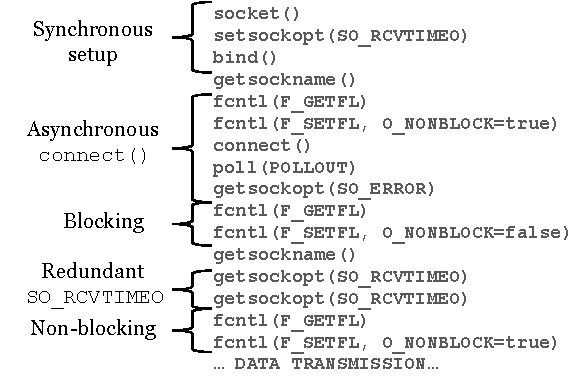
\includegraphics[width=\columnwidth]{figures/opening_pattern}
\caption{Opening pattern on TCP sockets. \textmd{After a synchronous setup
phase that binds the socket, a non-blocking connect() call is issued. After 2
redundant getsockopt(SO\_RCVTIMEO), the socket is turned in non-blocking mode
again before the transmission of data.}}
\label{fig:opening_pattern}
\end{figure}

Surprisingly, 15 applications use the
\texttt{listen()} call. Among those, only 11 ever accepted an incoming
connection with \texttt{accept()} or \texttt{accept4()}. Among the 449 incoming
connection observed, 98\% originated from a loopback address.
We noticed 5 connections originating from a link-local address while
3 connections originated from a remote network. These 3 remote incoming
connections were accepted by a single application, Skype, that uses NAT
traversal.

Let us now focus our analysis on the data transfer. 94\% of the TCP sockets
exchange data after the \texttt{connect()} call. Almost all
applications use the generic \texttt{read()} and \texttt{write()} calls.
Only half of them use their dedicated socket counterparts, \texttt{recv()} and
\texttt{send()}. Given the cost of issuing system calls, networking
textbooks recommend to use large buffers when transferring data.
\tcpsnitch allows to dissect how applications use each call.
Figure~\ref{fig:recv_buffers} shows a cumulative distribution function for the
size of the buffer given the the various receive functions. Surprisingly,
we observe that respectively 34\% and 16\% of the \texttt{recv()} and
\texttt{recvfrom()} calls use a buffer of exactly 1 byte and we also observe a
lot of 5 bytes long buffers. Overall, about half of the \texttt{recv()} calls
are passed a buffer of 5 bytes or less.

These functions support optional flags. The most popular sending flag is
\texttt{MSG\_NOSIGNAL} which is set on 60\% of the calls. This flag requests
not to send the \texttt{SIGPIPE} signal, which by default terminates the
process, when an application writes to a disconnected socket. It
is particularly useful for libraries since this flag does not modify
the process signal handlers. Only two other sending flags are used:
\texttt{MSG\_DONTWAIT} and \texttt{MSG\_MORE}. 13\% of the calls
are non-blocking thanks to the \texttt{MSG\_DONTWAIT} flag. 
\texttt{MSG\_MORE} is set on 2\% of the calls to indicate that more data is
coming. The other sending flags\footnote{\texttt{MSG\_CONFIRM},
\texttt{MSG\_DONTROUTE}, \texttt{MSG\_EOR} and \texttt{MSG\_OOB}} are never used.
18\% of the receiving calls are turned non-blocking using
the \texttt{MSG\_DONTWAIT} flag and 16\% of the calls set the
\texttt{MSG\_PEEK} flag to peek on the TCP receive queue without removing data.
Finally, a tiny fraction of those receiving calls (0.04\%) set
\texttt{MSG\_WAITALL} to request the operating system to block until it has
enough data to fill the buffer. The remaining flags\footnote{\texttt{MSG\_CMSG\_CLOEXEC},
\texttt{MSG\_ERRQUEUE}, \texttt{MSG\_OOB}, \texttt{MSG\_TRUNC}} do not
appear in our traces.

\begin{figure}
\centering
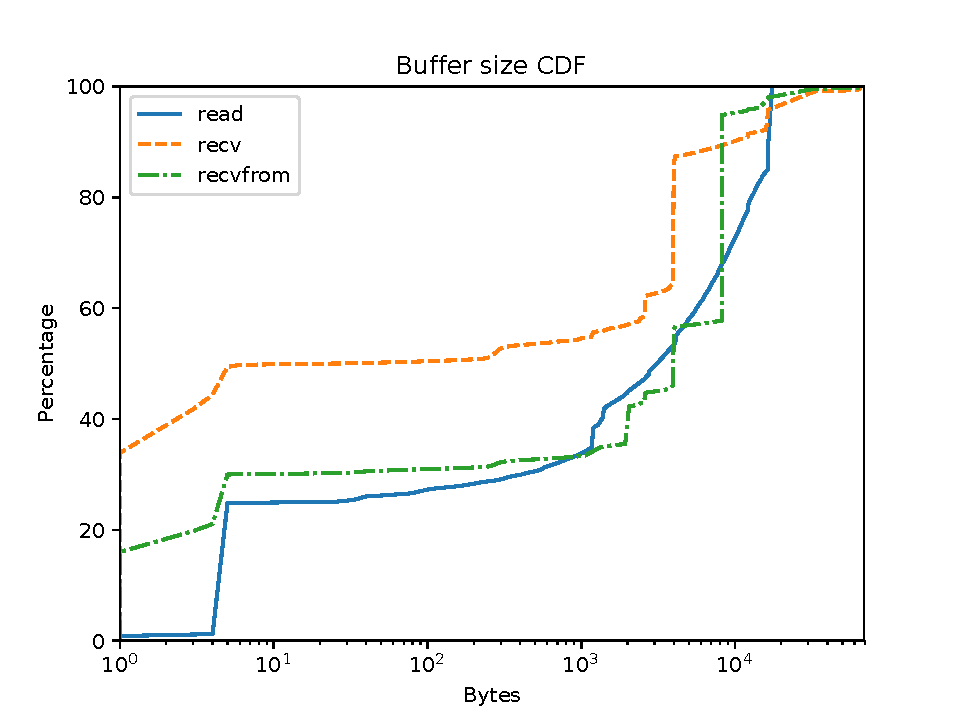
\includegraphics[width=\columnwidth]{figures/recv_buffers_log}
\caption{Cumulative distribution function of the buffer size passed to the
        different receive functions. Half of the recv() calls use a buffer of 5
        bytes or less.}
\label{fig:recv_buffers}
\end{figure}

As observed for the connection establishment, there is a very frequent pattern
for the termination of a connection. 78 applications and about half of all
opened sockets use \texttt{getsockopt(SO\_DEBUG)} and
\texttt{getsockopt(SO\_LINGER)} before issuing \texttt{close()}. The
utilization of \texttt{SO\_DEBUG} at this point of the connection is
surprising. We investigated the Android source code and confirmed its usage in
the IO Java core library of Android \cite{aosp_blockguardos} where a function
closes all file descriptors. Because sockets using \texttt{SO\_LINGER} need
some additional processing to avoid the socket API \texttt{close()} call to
block, a \texttt{getsockopt()} is issued to detect if the file descriptor is a
socket. If this call succeeds, then the file descriptor is indeed a socket.
It seems that a failed \texttt{getsockopt(SO\_DEBUG)} is less critical from a
performance viewpoint than a failed \texttt{getsockopt(SO\_LINGER)},
hence its use. This closing pattern would certainly be observed
on a much higher proportion of the sockets if \tcpsnitch
could terminate cleanly the traced Android applications.

\begin{figure}
\centering
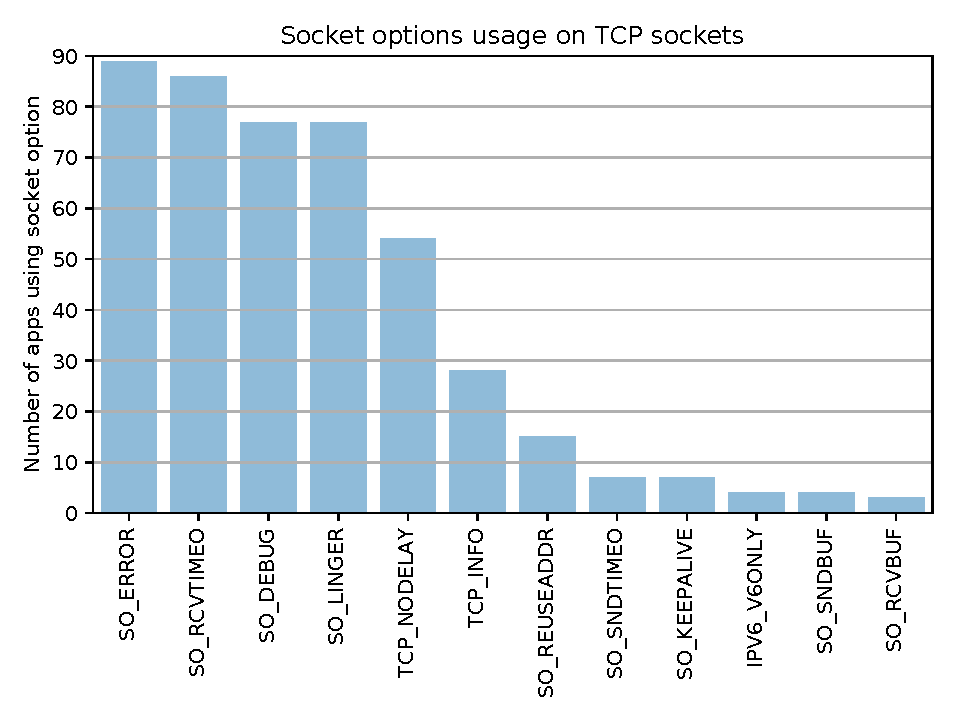
\includegraphics[width=\columnwidth]{figures/sockopts_bars}
\caption{Number of applications using each socket option.
    SO\_ERROR is often used after a non blocking
connect(). SO\_RCVTIMEO appears at the beginning of most TCP connections.
SO\_DEBUG and SO\_LINGER are used together before close(). TCP\_INFO
is used by a surprisingly large number of applications.}
\label{fig:sockopts_bars}
\end{figure}

\subsection{Socket options}

Socket options can be used by applications to tune the behavior of
the underlying TCP/IP stack. Linux supports a growing number of
non-standard socket options. Figure~\ref{fig:sockopts_bars} shows how many
applications use the main socket options observed in our dataset.
Several of these options are expected and some were discussed earlier,
\texttt{TCP\_INFO} was more surprising. This non-standard Linux TCP option
exports to the application counters maintained by the TCP stack. The standard
Android Java API does not expose this socket option and applications must
resort to a C/C++ library to use it. Still, 28 applications make use
of this socket option. As expected, those are mostly highly popular
applications such as Youtube, Chrome, Facebook or Spotify. For these
applications, \texttt{TCP\_INFO} was retrieved by 26\% of the
\texttt{SOCK\_STREAM} sockets and 73\% of these sockets retrieve
\texttt{TCP\_INFO} only once. Facebook, Messenger and Instagram are the
only applications that issue dozens of \texttt{TCP\_INFO} on a 
single TCP connection. For instance, we observed a Facebook TCP
connection lasting 32 seconds where \texttt{TCP\_INFO} was retrieved about
3000 times, almost as often as the 3500 \texttt{recv()} calls on the same
connection. These \texttt{TCP\_INFO} calls do not specifically happen at the
start or the end of a connection, but seem uniformly distributed during the
lifetime of the TCP connection.
